\documentclass[11pt]{article}
\usepackage[margin=0.95in]{geometry}
\usepackage{amsmath,amssymb,graphicx,booktabs}
\usepackage[T1]{fontenc}
\newcommand{\kF}{k_{\mathrm F}}
\newcommand{\vF}{v_{\mathrm F}}
\newcommand{\einf}{\epsilon_\infty}
\newcommand{\OK}{\Omega_K}
\newcommand{\Rs}{R_{\mathrm s}}
\begin{document}\sloppy
\begin{center}\large\textbf{Plasmon-mediated pairing in 2D lives at small scattering angles;\\
without them a critical coupling $\alpha_c\sim1$ appears}\end{center}

\section*{Summary}
The plasmon-pole interaction acts only for momentum transfers inside a window $q<K=a\kappa$
($\kappa=N\alpha\kF$ the screening momentum, $a\lesssim1$). At weak coupling every such
transfer is a small scattering angle,
\[
\phi\;\le\;\phi_K\equiv\frac{K}{\kF}=aN\alpha\;\ll\;1 .
\]
The argument has three steps.
\begin{enumerate}
\item The naive (BCS/Eliashberg ladder) gap equation has a solution at any $\alpha$,
$T_c\sim\OK e^{-c^2/\alpha^2}$, and this solution is built entirely from angles below
$\phi_K$ (Section~1).
\item Scattering at angles below $\phi_0=(\kF\Rs)^{-1/2}$ is the forward-scattering sector
that multidimensional bosonization treats exactly. There the pair correlator acquires only a
finite factor and no logarithm, so the ladder's Cooper logarithm from this sector is
spurious, and the sector is removed from the gap equation (Section~2). \emph{This is the
one physical assumption of the note.}
\item With angles below $\phi_0$ removed, the gap equation has no solution for
$\alpha<\phi_0/Na$ (the plasmon window lies entirely below $\phi_0$), and numerically
requires $\alpha\gtrsim1$ (Section~3). For $\Rs\sim1/\kappa$ this gives
$\alpha_c\gtrsim1/Na^2$.
\end{enumerate}
Numerical checks and technical details are collected in the Appendix.

\section*{1. The naive gap equation and the angles it uses}

\paragraph{Setup.}
$\alpha=e^2/\einf\vF$, $N$ flavours, $\kappa=N\alpha\kF$, plasmon
$\Omega_q^2=\tfrac12\kappa\vF^2q$. The plasmon-pole interaction, valid for $|\nu|>\vF q$, is
\begin{equation}
U(i\nu,q)=\frac{2\pi e^2}{\einf q}\,\frac{\nu^2}{\nu^2+\Omega_q^2}\;\theta(|\nu|-\vF q),
\qquad q<K=a\kappa ,
\label{eq:U}
\end{equation}
and the linearized $T=0$ gap equation ($\mathbf k$ on the Fermi surface) is
\begin{equation}
\Delta(w)=-\int\!\frac{dw'}{2\pi}\int\!\frac{d^2p}{(2\pi)^2}\,
U(w-w',|\mathbf k-\mathbf p|)\,\frac{\Delta(w')}{w'^2+\xi_p^2}.
\label{eq:gap}
\end{equation}
Units $\vF=\kappa=1$: then $e^2/\einf=\alpha$, $\Omega_q^2=q/2$, $K=a$, $\OK^2=a/2$, and
$\kF=1/N\alpha\gg1$.

\paragraph{1.1 Reduction to a one-dimensional $q$-integral.}
Write $p=\kF+\xi$ and let $\phi$ be the angle between $\mathbf p$ and $\mathbf k$. For small
angles $q^2\simeq\xi^2+\kF^2\phi^2$ and $d^2p\simeq\kF\,d\xi\,d\phi$. At fixed $\xi$
substitute $\phi\to q$ ($\kF\,d\phi=q\,dq/\sqrt{q^2-\xi^2}$, two branches $\pm\phi$),
exchange the order of integration and set $\xi=q\sin\theta$:
\begin{equation}
\int\!\frac{d^2p}{(2\pi)^2}\,\frac{U(\nu,q)}{w'^2+\xi^2}
=\frac{1}{2\pi^2}\int_0^{K}\!dq\,q\,U(\nu,q)\int_{-q}^{q}\frac{d\xi}{(w'^2+\xi^2)\sqrt{q^2-\xi^2}}
=\frac{1}{2\pi}\int_0^{K}\!dq\,\frac{q\,U(\nu,q)}{|w'|\sqrt{w'^2+q^2}} .
\label{eq:exact}
\end{equation}
The condition $|\nu|>q$ involves only the full transfer $q$, so it just lowers the upper limit
to $q_{\max}(\nu)=\min(K,|\nu|)$. With $qU=2\pi\alpha\,\nu^2/(\nu^2+\Omega_q^2)$:
\begin{equation}
\boxed{\;\Delta(w)=-\frac{\alpha}{2\pi}\int dw'\int_0^{q_{\max}(\nu)}\!dq\,
\frac{\nu^2}{\nu^2+\Omega_q^2}\;\frac{\Delta(w')}{|w'|\sqrt{w'^2+q^2}},
\qquad\nu=w-w'.\;}
\label{eq:red}
\end{equation}

\paragraph{1.2 What $q$ means in terms of angles.}
At fixed $q$ the angle is $|\phi|=\sqrt{q^2-\xi^2}/\kF$: it equals $q/\kF$ on shell
($\xi=0$) and goes to zero for $|\xi|\to q$. Two consequences:
\begin{itemize}
\item[(a)] Every term of (\ref{eq:red}) has $|\phi|\le q/\kF\le\phi_K=aN\alpha$, on shell and
off shell alike. The whole equation is small-angle scattering.
\item[(b)] After the $\xi$-integration a given $q$ contains \emph{all} angles from $0$ to
$q/\kF$. A lower cut on $q$ is therefore not a lower cut on the angle; an angular cut has to
be imposed before the $\xi$-integration (Section~3.1).
\end{itemize}

\paragraph{1.3 The solution is built from the smallest angles.}
The kernel of (\ref{eq:red}) is positive, so a solution must change sign in frequency
(Tolmachev--Anderson). Projecting on a low-frequency block (below $\simeq0.3\,\OK$) and a
high-frequency block gives the condition $\alpha^2M\ln(\OK/E)\simeq1$, with $E$ the
infrared scale: a solution exists for any $\alpha$, with $T_c\sim\OK e^{-c^2/\alpha^2}$
($c\simeq2.7$ at $a=0.3$; previous note). The logarithm is the Cooper logarithm of transfers
inside the window, i.e.\ of angles below $\phi_K$. Figure~\ref{fig:phi}b makes this
quantitative: removing the angles $|\phi|<q_f/\kF$ (Section~3.1) and recomputing the pairing
eigenvalue $\mu$: removing the angles below $0.1\,\phi_K$ already reduces $|\mu|$ by $35\%$,
below $0.45\,\phi_K$ by a factor $4.5$, below $0.85\,\phi_K$ by a factor $30$.

\section*{2. Why the small-angle sector is removed}

The Cooper ladder is the correct resummation (equivalent to one-loop RG in the Cooper
channel) for an interaction that transfers momenta of order $\kF$. Equation (\ref{eq:red}) is
a ladder for an interaction whose transfers are all $\le aN\alpha\,\kF$. For such forward
scattering an exact treatment exists, and it gives a different answer.

\paragraph{2.1 The forward-scattering sector.}
Let $\Rs$ be the range of the interaction ($q\lesssim1/\Rs$). Divide the Fermi surface into
patches and linearize the dispersion on each: a state at angle $\phi$ from the patch centre
has the curvature energy $\kF^2\phi^2/2m$, which is negligible against the energy scale
$\vF/\Rs$ probed by the interaction when
\begin{equation}
\phi\ll\phi_0\equiv\frac{1}{\sqrt{\kF\Rs}} .
\label{eq:phi0}
\end{equation}
Inside such flat patches the density on each patch is a free boson and the interaction is
quadratic in the bosons: the sector of scattering angles $|\phi|\lesssim\phi_0$ is exactly
solvable (multidimensional bosonization). For $\Rs\sim1/\kappa$,
$\phi_0\sim\sqrt{N\alpha}$, parametrically larger than $\phi_K=aN\alpha$.

\paragraph{2.2 The pair correlator in this sector.}
A fermion on patch $n$ is $\psi_n\propto e^{i\Phi_n}$, so the pair operator on opposite
patches, $P=\psi_n\psi_{\bar n}$, has the exact correlator
\begin{equation}
\chi_P(x,\tau)=\chi_P^{(0)}(x,\tau)\,e^{-Q_P(x,\tau)},\qquad
Q_P=Q_{nn}+Q_{\bar n\bar n}+2Q_{n\bar n},
\label{eq:DW}
\end{equation}
\begin{equation}
Q_{nm}(x,\tau)=\int\!\frac{d^2q}{(2\pi)^2}\frac{d\nu}{2\pi}\,
\frac{V(q,i\nu)\,[1-\cos(\mathbf q\cdot\mathbf x-\nu\tau)]}
{(i\nu-\mathbf v_n\!\cdot\!\mathbf q)(i\nu-\mathbf v_m\!\cdot\!\mathbf q)} .
\label{eq:Qnm}
\end{equation}
The question is whether $Q_P$ grows logarithmically at large $x,\tau$ (which would be the
counterpart of the Cooper logarithm) or saturates. In the plasmon window $|\nu|>q$ both
denominators are $\simeq-\nu^2$, the four terms add, and at large distance
\begin{equation}
|Q_P^{\rm (pl)}|\simeq\frac{4\alpha}{\pi}\int_0^{K}\frac{dq}{\Omega_q}
\arctan\frac{\Omega_q}{q}\;\le\;4\sqrt2\,\alpha\sqrt a ,
\label{eq:Qpl}
\end{equation}
numerically $|Q_P|=2.4\,\alpha$ for $a=0.3$. The integral converges at small $q$ because
$\int d\nu/(\nu^2+\Omega_q^2)\propto q^{-1/2}$. There is no logarithm: forward scattering in
the plasmon window multiplies the pair bubble by a constant $1+O(\alpha\sqrt a)$.

\paragraph{2.3 Consequence, and what is assumed.}
The ladder over the same sector produces $\ln(\OK/E)$ and $T_c\sim e^{-c^2/\alpha^2}$; the
exact treatment produces a finite factor. We therefore remove the angles $|\phi|<\phi_0$
from the gap equation and keep the ladder only for $|\phi|>\phi_0$. Two points are not
settled here: (i) the static part of the sector, $|\nu|<\vF q$, is not included in
(\ref{eq:Qpl}); for a static repulsion the known result is a power-law \emph{suppression}
of $\chi_P$ (Miserev, Schoeller, Klinovaja, Loss, arXiv:2312.17208), which cannot help
pairing; (ii) $\phi_0$ is defined only up to a factor of order one. Section~3 therefore
treats $\phi_0$ as a free parameter.

\section*{3. Gap equation without the small-angle sector}

\paragraph{3.1 The angular cut.}
By 1.2(b) the cut $|\phi|>\phi_0$ must be imposed in the $(\xi,\phi)$ variables. With
$q^2=\xi^2+\kF^2\phi^2$ it reads $q^2>\xi^2+q_f^2$, where
\begin{equation}
q_f\equiv\kF\phi_0=\frac{\phi_0}{N\alpha}\qquad\text{(units of $\kappa$)} .
\label{eq:qf}
\end{equation}
Exchanging the order of integration, this is $q>q_f$ \emph{and} $|\xi|<b(q)\equiv\sqrt{q^2-q_f^2}$.
The $\xi$-integral of (\ref{eq:exact}) over the reduced range is again elementary:
\begin{equation}
\int_{-b}^{b}\frac{d\xi}{(w'^2+\xi^2)\sqrt{q^2-\xi^2}}
=\frac{2}{|w'|\sqrt{w'^2+q^2}}\arctan\!\Big(\frac{\sqrt{w'^2+q^2}}{|w'|}\,\frac{b}{q_f}\Big).
\label{eq:arctan}
\end{equation}
This is exact within the small-angle kinematics (Appendix~A.1), and gives $\pi/|w'|\sqrt{w'^2+q^2}$
for $q_f\to0$. The factor $\frac2\pi\arctan(\cdot)$ is the fraction of weight that survives
the cut. In the Cooper regime $|w'|\ll q$ it is $\simeq1$: the relevant states are on shell,
and the angle cut acts like a plain cut $q>q_f$. In the plasmon regime $|w'|\gg q$ it is
$\frac2\pi\arccos(q_f/q)<1$: off-shell states at small angle are also removed. The gap equation
becomes
\begin{equation}
\boxed{\;\Delta(w)=-\frac{\alpha}{2\pi}\int dw'\int_{q_f}^{q_{\max}(\nu)}\!dq\,
\frac{\nu^2}{\nu^2+\Omega_q^2}\;
\frac{2}{\pi}\arctan\!\Big(\frac{\sqrt{w'^2+q^2}\sqrt{q^2-q_f^2}}{|w'|\,q_f}\Big)
\frac{\Delta(w')}{|w'|\sqrt{w'^2+q^2}}.\;}
\label{eq:ang}
\end{equation}
Since the cut is fixed in angle, $q_f$ depends on $\alpha$ through (\ref{eq:qf}).

\paragraph{3.2 Exact bound: the window must be open.}
Equation (\ref{eq:ang}) has an empty $q$-range unless $q_f<K$, i.e.
\begin{equation}
\boxed{\;\alpha\;>\;\alpha_{\min}(\phi_0)=\frac{\phi_0}{Na}\;}
\label{eq:bound}
\end{equation}
For smaller $\alpha$ every plasmon transfer is an angle below $\phi_0$: the whole window
lies in the forward-scattering sector and nothing is left for the ladder.

\paragraph{3.3 Numerical solution.}
Equation (\ref{eq:ang}) is written as $\Delta=-\alpha A\Delta$ and the lowest eigenvalue
$\mu$ of $A$ gives $\alpha=-1/\mu$. Since $A$ depends on $\alpha$ only through $q_f$, we
compute $\mu(q_f)$ and read the critical coupling from $\alpha_c=-1/\mu(q_f)$,
$\phi_0=N\alpha_c q_f$ (Fig.~\ref{fig:phi}a and the table; $N=2$, $E$ in units of
$\kappa\vF$).

\begin{center}
\begin{tabular}{lcccc}
\toprule
$\alpha_c$ ($N=2$) & $\phi_0=0.05$ & $0.1$ & $0.2$ & $0.3$\\
\midrule
$a=0.3$, $E=10^{-4}$ & 1.19 & 1.42 & 1.78 & 2.08\\
$a=0.3$, $E=10^{-6}$ & 0.93 & 1.15 & 1.48 & 1.76\\
$a=0.3$, $E=10^{-8}$ & 0.81 & 1.01 & 1.32 & 1.59\\
$a=1.0$, $E=10^{-4}$ & 0.77 & 0.87 & 1.03 & 1.16\\
$a=1.0$, $E=10^{-6}$ & 0.60 & 0.70 & 0.84 & 0.96\\
$a=1.0$, $E=10^{-8}$ & 0.51 & 0.61 & 0.74 & 0.86\\
bound (\ref{eq:bound}), $a=0.3$ & 0.08 & 0.17 & 0.33 & 0.50\\
bound (\ref{eq:bound}), $a=1.0$ & 0.025 & 0.05 & 0.10 & 0.15\\
\bottomrule
\end{tabular}
\end{center}

\begin{figure}[t]
\centering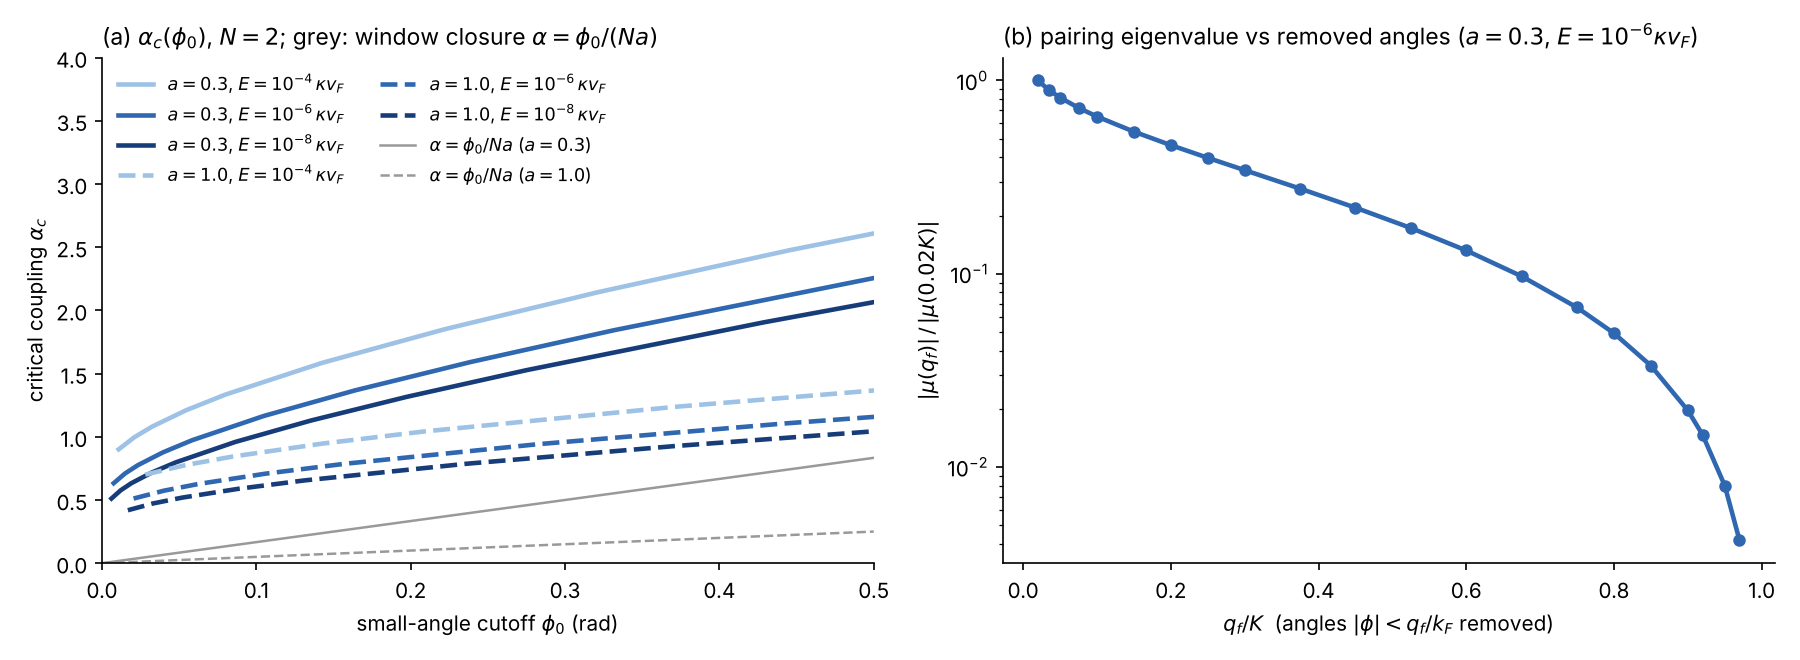
\includegraphics[width=\textwidth]{alphac_phi0.png}
\caption{(a) Critical coupling of (\ref{eq:ang}) versus the small-angle cutoff $\phi_0$
($N=2$; two window sizes $a$, three infrared scales $E$), plotted parametrically,
$\alpha_c=-1/\mu(q_f)$, $\phi_0=N\alpha_c q_f$. Grey: the exact bound (\ref{eq:bound}).
(b) Pairing eigenvalue of the naive equation (\ref{eq:red}) with the angles
$|\phi|<q_f/\kF$ removed, relative to $q_f=0.02K$ ($a=0.3$, $E=10^{-6}\kappa\vF$).}
\label{fig:phi}
\end{figure}

What the numbers say: (i) $\alpha_c$ is of order one for any reasonable $\phi_0$
($0.6$--$1.4$ at $\phi_0=0.1$). (ii) $\alpha_c$ grows slowly with $\phi_0$ (roughly
$\phi_0^{1/3}$) and decreases with the window size (roughly $a^{-1/2}$). (iii) $\alpha_c$
still decreases with $E$: for angles between $\phi_0$ and $\phi_K$ the ladder is legitimate,
the Cooper logarithm is real, and $\alpha_c\to\alpha_{\min}$ as $E\to0$. But this happens only
like $[\ln(\OK/E)]^{-1/2}$: at $\phi_0=0.1$, $a=0.3$ the bound is $0.17$ while
$\alpha_c=1.0$ at $E=10^{-8}$.

\paragraph{3.4 The screened Coulomb case.}
With $\Rs\sim1/\kappa$, $\phi_0\sim\sqrt{N\alpha}$ and the bound (\ref{eq:bound}) becomes a
condition on $\alpha$ alone, $\alpha>\sqrt{N\alpha}/Na$, i.e.
\begin{equation}
\alpha_c\gtrsim\frac{1}{Na^2},
\end{equation}
which is $0.5$ for $N=2$, $a=1$ and $5.6$ for $a=0.3$. Equivalently, at weak coupling
$\phi_K=aN\alpha\ll\sqrt{N\alpha}=\phi_0$: the entire plasmon window is forward scattering.

\section*{Conclusion}
The weak-coupling solution of the plasmon gap equation is a Cooper logarithm produced by
forward scattering, $\phi\le aN\alpha$. Treating that sector exactly instead of by the ladder
removes it; what remains has no solution below $\alpha_{\min}=\phi_0/Na$ and in practice
requires $\alpha_c\simeq1$, where the one-loop treatment is no longer controlled.
Plasmon-mediated superconductivity at weak coupling is excluded, given the assumption of
Section~2.

\appendix
\section*{Appendix: checks and numerical details}

\paragraph{A.1 Angular cut, Eq.~(\ref{eq:arctan}).}
Equation (\ref{eq:arctan}) inserted into (\ref{eq:exact}) was compared with a direct
two-dimensional integration over $(\xi,\phi)$ with $|\phi|>\phi_0$ imposed literally, with the
small-angle kinematics and with the exact ones, $q^2=\xi^2+2\kF(\kF+\xi)(1-\cos\phi)$,
measure $(\kF+\xi)\,d\xi\,d\phi$ ($\kF=5\kappa$, \texttt{check\_phi\_cut.py}):
\begin{center}\small
\begin{tabular}{cccc|cccc}
\toprule
$w'$ & $\nu$ & $\phi_0$ & $q_{\max}$ & direct, exact & direct, small-angle & Eq.~(\ref{eq:arctan}) & plain $q>q_f$\\
\midrule
0.3 & 0.8 & 0.02 & 0.3 & 1.02463 & 1.02454 & 1.02454 & 1.605\\
0.2 & 0.9 & 0.05 & 0.3 & 0.24429 & 0.24368 & 0.24368 & 0.629\\
0.02 & 0.3 & 0.03 & 0.25 & 10.7335 & 10.7306 & 10.7306 & 12.24\\
0.01 & 0.5 & 0.02 & 0.3 & 76.5619 & 76.5479 & 76.5479 & 80.92\\
0.001 & 0.5 & 0.04 & 0.3 & 270.434 & 270.303 & 270.303 & 271.93\\
\bottomrule
\end{tabular}\normalsize
\end{center}
With the small-angle kinematics the agreement is to $10^{-15}$; the exact kinematics differ by
at most $2.5\times10^{-3}$ (curvature, relative order $q/\kF$). A plain lower cut on $q$
is wrong by up to a factor $2.6$ in the plasmon regime. In the gap equation the difference is
quantitative: at $a=0.3$, $E=10^{-6}$, $q_f=0.1K$ ($0.3K$) the angle cut gives
$\alpha=0.97$ ($1.84$), the $q$-cut $0.87$ ($1.47$).

\paragraph{A.2 The plasmon condition.}
Replacing $\theta(|\nu|-\vF q)$ by the upper limit $q_{\max}(\nu)$ in (\ref{eq:red}) is exact,
because the condition involves only the full transfer $q$ and not $\xi$ or $\phi$ separately. The condition is on the
transfer frequency $\nu$, not on $w'$: pairs with $|w'|\ll\vF q$ exchanging a plasmon with
$|\nu|\gg\vF q$ are inside the validity domain.

\paragraph{A.3 Numerics.}
Logarithmic frequency grid from $E$ to $10\,\OK$ ($34$ points per decade, $\Delta$ even in
$w$), Gauss--Legendre in $q$ after $q=|w'|\sinh t$ (140 nodes); grid errors are below
$10^{-4}$. Raising the frequency cutoff from $10\,\OK$ to $30\,\OK$ changes $\mu$ by $3\%$.
Table entries solve $\alpha\,\mu(\phi_0/N\alpha)=-1$ directly at fixed $\phi_0$
(\texttt{solve\_angular\_cutoff.py}, \texttt{make\_alphac.py}).
\end{document}
